% !TeX root = ../report.tex
% Chapter 2: Related theory and works
\chapter{ทฤษฎีความรู้และงานที่เกี่ยวข้อง}
\thaijustify{
  ในบทที่ 2 นี้จะกล่าวถึงทฤษฎีที่เกี่ยวข้องที่ใช้ในการทำงานและการศึกษาเพื่อบรรลุวัตถุประสงค์ อธิบายคำศัพท์หรือภาษาทาง
  คอมพิวเตอร์ เทคโนโลยีที่จะนำมาประยุกต์ใช้งานและแก้ปัญหาต่าง ๆ ในโครงงาน รวมไปถึงงานวิจัย ผลิตภัณฑ์ หรือโครงงานที่นำมาใช้อ้างอิง เพื่อนำมาสังเคราะห์เป็นกรอบแนวคิดในการแก้ปัญหาและกำหนดขอบเขตของโครงงาน
}

\section{ทฤษฎีที่เกี่ยวข้อง}

\subsection{UX/UI Development Life Cycle: UX/UI DLC}
\thaijustify{
  กระบวนการออกแบบประสบการณ์ผู้ใช้และส่วนต่อประสานผู้ใช้เป็นกระบวนการที่เน้นผู้ใช้เป็นศูนย์กลางและต้องอาศัยการทำซ้ำอย่างต่อเนื่อง (Iterative process) โดยทั่วไปนักออกแบบจะต้องผ่านขั้นตอนตั้งแต่การรวบรวมความต้องการ การทำความเข้าใจผู้ใช้ (Empathize) การระบุปัญหา (Define) การระดมความคิด (Ideate) การสร้างต้นแบบ (Prototype) และการทดสอบ (Test)
}
\thaijustify{
  อย่างไรก็ตาม ในทางปฏิบัตินักออกแบบมักเผชิญข้อจำกัดด้านเวลาและทรัพยากร
  ทำให้การสำรวจแนวคิด การรับข้อเสนอแนะ และการปรับปรุงงานซ้ำหลายรอบทำได้ไม่เต็มที่
  Suh et al. \cite{suh2025storyensemble} ชี้ให้เห็นว่าข้อจำกัดดังกล่าวลดโอกาสในการสำรวจทางเลือกและย้อนกลับไปปรับแก้งานในขั้นตอนก่อนหน้า ขณะที่
  Feng et al. \cite{feng2023designing} แสดงให้เห็นว่าการสร้าง wireframe
  ด้วยมือเป็นงานที่ใช้เวลาและแรงงาน ซึ่งสามารถใช้ LLM ช่วยสร้าง wireframe
  จากความต้องการทางการออกแบบได้ และ Yuan et al. \cite{prototypeflow_humanai_ui_design} พบว่าการสร้าง
  UI ด้วย Generative AI ควรเปิดโอกาสให้นักออกแบบตรวจสอบและปรับผลลัพธ์ระหว่างกระบวนการ
  แทนการสร้างผลลัพธ์เพียงครั้งเดียว
}

\thaijustify{จากงานเหล่านี้จึงเห็นได้ว่า Generative AI สามารถช่วยลดภาระของงานที่ต้องทำ
  ด้วยมือและสนับสนุนกระบวนการออกแบบแบบวนซ้ำ ทำให้นักออกแบบมีเวลาสำหรับการทดสอบกับผู้ใช้และนำข้อเสนอแนะกลับมาปรับปรุงต้นแบบได้มากขึ้น
}

\subsection{ระเบียบวิธีการทดสอบการใช้งาน (Usability test)}
\thaijustify{
  การทดสอบกับผู้ใช้เป็นหัวใจสำคัญในการหาข้อบกพร่องและข้อควรปรับปรุงของงานออกแบบ
  โดยงานวิจัยชี้ให้เห็นว่าการทดสอบบ่อยครั้งกับกลุ่มตัวอย่างขนาดเล็กให้ข้อมูลเชิงลึกที่นำไปปรับปรุงได้จริงมากกว่าการทดสอบสเกลใหญ่แต่นาน ๆ ครั้ง โดย Nielsen \cite{nielsen2000five} เสนอว่า
  การทดสอบเชิงคุณภาพสามารถเริ่มต้นด้วยผู้เข้าร่วมประมาณ 5 คนต่อรอบ เนื่องจากภายใต้
  แบบจำลองการค้นพบปัญหาด้านการใช้งาน ผู้เข้าร่วม 5 คนสามารถค้นพบปัญหาได้ประมาณ
  ร้อยละ 85 และการเพิ่มผู้เข้าร่วมหลังจากนั้นมีแนวโน้มให้ข้อมูลใหม่ลดลงด้วย จึงควรนำผลที่ได้
  ไปปรับปรุงต้นแบบและทดสอบซ้ำในรอบถัดไป
  แนวคิดนี้สอดคล้องกับ Virzi \cite{virzi1992refining} ซึ่งพบว่าผู้เข้าร่วมประมาณ 4-5 คนสามารถค้นพบปัญหา
  ด้านการใช้งานได้ประมาณร้อยละ 80  และแบบจำลองของ
  Nielsen และ Landauer \cite{nielsen1993mathematical} ที่แสดงให้เห็นว่าประโยชน์จากการเพิ่มจำนวนผู้เข้าร่วมจะลดลง
  เรื่อย ๆ เมื่อปัญหาส่วนใหญ่ถูกค้นพบแล้ว อย่างไรก็ตาม จำนวนดังกล่าวเหมาะสำหรับการทดสอบเชิงคุณภาพเพื่อค้นหาปัญหาและปรับปรุงงานแบบวนซ้ำ ไม่ใช่เกณฑ์ตายตัวสำหรับการทดสอบทุกประเภท ใน UX/UI DLC มีระเบียบวิธีทดสอบการใช้งานที่นิยมใช้ ดังนี้
  \begin{itemize}
    \item \textbf{Usability Test} เป็นการทดสอบเพื่อให้ผู้เข้าร่วมทดสอบลองใช้งานระบบและหาจุดที่ใช้งานยากหรือติดขัด ซึ่งในขณะที่ทำการทดสอบผู้เข้าร่วมทดสอบจำเป็นต้องคิดไปด้วยพูดไปด้วย (Thinking-Aloud) โดยนักออกแบบจะคอยสังเกตพฤติกรรมและรับฟังความคิดเห็นของผู้เข้าร่วมทดสอบขณะทำภารกิจที่กำหนด \cite{rubin2008handbook, dumas1999practical, nielsen1993usability}
    \item \textbf{A/B Test} เป็นกระบวนการนำเสนอทางเลือกการออกแบบ (Variants) ที่แตกต่างกันให้กับผู้ใช้ เพื่อเปรียบเทียบประสิทธิภาพการใช้งานและรวบรวมข้อเสนอแนะก่อนที่จะตัดสินใจออกแบบในขั้นตอนถัดไป ในภาคอุตสาหกรรม A/B Test มักหมายถึงการทดลองแบบควบคุมบนระบบจริง (Online Controlled Experiment) ที่วัดผลด้วยสถิติโดยเมทริกซ์ต่าง ๆ เช่น conversion rate, click-throughs rate, task completion rate จากผู้ใช้จำนวนมาก \cite{kohavi2009controlled, kohavi2020trustworthy} อย่างไรก็ตาม วิธีนี้ให้ผลเป็นตัวเลขว่าทางเลือกใดทำงานได้ดีกว่า แต่ไม่อธิบายเหตุผลเบื้องหลังพฤติกรรมของผู้ใช้ จึงควรใช้ร่วมกับการรวบรวมข้อมูลเชิงคุณภาพ \cite{nielsen2005abtesting} % ในโครงงานนี้ A/B Test หมายถึงการให้ผู้ใช้กลุ่มเล็กลองใช้ต้นแบบสองรูปแบบและให้ข้อเสนอแนะในแต่ละรอบการทดสอบ ซึ่งเป็นแนวทางเชิงคุณภาพ
    \item \textbf{Comparative Usability Test} มีหลักการคล้าย A/B Test แต่เน้นการทดสอบเชิงคุณภาพและให้ผู้ใช้เปรียบเทียบดีไซน์ตั้งแต่สองรูปแบบขึ้นไปที่มีเป้าประสงค์เดียวกัน งานวิจัยพบว่าการให้ผู้ใช้เห็นทางเลือกการออกแบบหลายแบบพร้อมกันช่วยให้ผู้ใช้ให้ความคิดเห็นได้เปิดกว้างและลึกกว่าการทดสอบการใช้งานจากดีไซน์แบบเดียว~\cite{tohidi2006getting} อีกทั้งการสร้างต้นแบบหลายแบบยังนำไปสู่ผลงานที่ดีขึ้นและมีความหลากหลายของแนวคิดมากขึ้น~\cite{dow2010parallel}
  \end{itemize}
  จากการศึกษาข้างต้น โครงงานนี้เลือกใช้ \textit{Comparative Usability Test}
  เป็นหลัก โดยให้ผู้เข้าร่วมทดสอบเปรียบเทียบ two-alternative UI และให้ข้อเสนอแนะในแต่ละรูปแบบ เนื่องจากโครงงานนี้มุ่งเน้นการค้นหาปัญหาและความต้องการของผู้ใช้จากต้นแบบ เพื่อนำข้อเสนอแนะที่ได้กลับไปปรับปรุงการออกแบบในรอบถัดไป
  ทั้งนี้ Generative AI จะถูกนำมาใช้เพื่อช่วยสร้าง two-alternative UI รวบรวม
  และวิเคราะห์ข้อเสนอแนะ เพื่อลดภาระงานของนักออกแบบในการทดสอบแต่ละรอบ
}

\subsection{การสกัดความต้องการและการสร้าง User Persona จากข้อเสนอแนะของผู้ใช้}
\thaijustify{
  การทำความเข้าใจความต้องการของผู้ใช้เป็นส่วนสำคัญของกระบวนการออกแบบ
  โดยการใช้ต้นแบบเป็นหนึ่งในวิธีที่ช่วยให้นักออกแบบสามารถสกัดความต้องการ
  และรับข้อเสนอแนะจากผู้ใช้ได้ก่อนการพัฒนาระบบจริง \cite{pacheco2018}
  UI prototype  ยังใช้ทดสอบ ประเมิน และยืนยันแนวคิดร่วมกับผู้ใช้และทีมพัฒนาได้~\cite{kolthoff2024}โครงงานนี้เลือกใช้ต้นแบบระดับ high-fidelity เพื่อให้ผู้เข้าร่วมทดสอบสามารถชี้ข้อเสนอแนะไปยัง component ที่ต้องการได้โดยตรง ข้อมูลที่ได้จากการทดสอบต้นแบบจึงสามารถนำมาใช้เพื่อค้นหาปัญหาการใช้งาน ความต้องการ และความแตกต่างระหว่างผู้ใช้แต่ละกลุ่มได้
 
}
\thaijustify{
  อย่างไรก็ตาม ข้อเสนอแนะจากผู้ใช้ไม่ควรถูกตีความว่าเป็นปัญหาการใช้งาน
  หรือความต้องการโดยตรงทั้งหมด เนื่องจากความชอบของผู้ใช้อาจไม่สอดคล้อง
  กับประสิทธิภาพการใช้งานเสมอไป \cite{nngroup_satisfaction} และการใช้ผลการโหวตจากผู้เข้าร่วมจำนวนไม่มากเป็นข้อมูลเชิงปริมาณ อาจทำให้เกิดความเข้าใจผิดได้ \cite{nngroup_qualitative} นอกจากนี้ ข้อเสนอแนะจากผู้มีส่วนได้ส่วนเสียในแต่ละกลุ่มอาจมีความสำคัญแตกต่างกันตามบทบาท ความต้องการ ความเร่งด่วน และอิทธิพลต่อโครงการ \cite{shukla2025,mitchell1997} ดังนั้น การวิเคราะห์ข้อเสนอแนะจึงควรพิจารณาทั้งเนื้อหาของข้อเสนอแนะและบริบทของกลุ่มผู้ให้ข้อเสนอแนะร่วมกัน
}
\thaijustify{
  วิธีหนึ่งในการนำข้อมูลดังกล่าวมาใช้สนับสนุนกระบวนการออกแบบคือ
  User Persona ซึ่งเป็นตัวแทนของกลุ่มผู้ใช้ที่สร้างขึ้นจากข้อมูลของผู้ใช้
  เพื่อสรุปลักษณะและความต้องการที่สำคัญของแต่ละกลุ่ม งานของ
  Shin et al. \cite{shin2024} ศึกษาการใช้ Large Language Models
  ร่วมกับมนุษย์ในการสร้าง Persona จากข้อมูลผู้ใช้ ซึ่งพบว่าการให้ LLM
  สร้าง Persona จากข้อมูลทั้งหมดโดยอัตโนมัติยังมีข้อจำกัดในการระบุลักษณะสำคัญของกลุ่มผู้ใช้ ในทางกลับกัน การให้มนุษย์มีส่วนร่วมในการ
  ระบุและจัดกลุ่มข้อมูลตามลักษณะที่สำคัญ แล้วใช้ LLM ช่วยสรุปข้อมูลของแต่ละกลุ่มเป็น Persona สามารถสร้าง Persona ที่เป็นตัวแทนของข้อมูลผู้ใช้ได้ดีกว่า แนวทางดังกล่าวจึงสนับสนุนแนวคิด Human-in-the-loop
  แทนการให้ Generative AI เป็นผู้กำหนด Persona เพียงอย่างเดียว
}
\thaijustify{
  จากแนวคิดดังกล่าว โครงงานนี้จึงนำข้อเสนอแนะที่ได้จาก Comparative Usability Test มาใช้เป็นข้อมูลเชิงคุณภาพ โดยแยกพิจารณาปัญหาการใช้งาน ความชอบ และกลุ่มของผู้ให้ข้อเสนอแนะ จากนั้นใช้ Generative AI ช่วยรวบรวมและสรุปลักษณะร่วมของข้อมูลเพื่อสนับสนุนการสร้าง User Persona โดยให้นักออกแบบเป็นผู้ตรวจสอบและยืนยันการจัดกลุ่มและผลลัพธ์ที่ได้ Persona ที่ผ่านการตรวจสอบแล้วจึงสามารถใช้เป็นตัวแทนของความต้องการของผู้ใช้แต่ละกลุ่ม และเป็นข้อมูลประกอบการตัดสินใจในการปรับปรุง two-alternative UI ในรอบการออกแบบถัดไปได้
}

\subsection{ข้อกำหนดระบบการออกแบบด้วย Generative AI}
\thaijustify{
  การทำงานกับ Generative AI เพื่อสร้าง two-alternative UI จำเป็นต้องมีกรอบควบคุม (Guardrails) เพื่อให้ผลลัพธ์ที่ได้สอดคล้องกับอัตลักษณ์ของผู้ว่าจ้างหรือผลิตภัณฑ์นั้น ๆ Figma \cite{figma_agent} ระบุว่าการใช้ Design System ช่วยเป็นกรอบให้ Generative AI สามารถสร้างทางเลือกการออกแบบที่ถูกต้องได้ และ Design Tokens Community Group \cite{designtokens2025} ได้กำหนดมาตรฐานรูปแบบไฟล์สำหรับการแลกเปลี่ยน Design tokens ระหว่างเครื่องมือไว้ โครงงานนี้จึงกำหนดให้ Design System เป็นข้อบังคับใช้ควบคุมในการสร้าง UI ด้วย Generative AI และใช้ตรวจสอบความถูกต้องก่อนการส่งมอบ
}
% /2.1.6 - 2.2.3 เอามารวมกันเลย
\section{โครงงาน งานวิจัยหรือผลิตภัณฑ์ที่เกี่ยวข้อง}

\subsection{การสร้าง UI และวิเคราะห์ข้อเสนอแนะด้วย Generative AI}

\thaijustify{
  งานวิจัยด้านการสร้าง UI ด้วย LLM แสดงให้เห็นทั้งศักยภาพและข้อจำกัดของเทคโนโลยี โดย Kolthoff et al. \cite{kolthoff2024} พบว่าการสร้าง UI ยังมีข้อผิดพลาดด้านการจัดวาง การตีความฟังก์ชัน และความไม่สอดคล้องขององค์ประกอบ เช่น สี ตัวอักษร และรูปแบบของ component ขณะที่ Ataei et al. \cite{ataei2025} ใช้ LLM Agents จำลองผู้ใช้เพื่อค้นหาความต้องการที่ไม่ได้ถูกระบุโดยตรง แต่ยังไม่ได้มุ่งเน้นการทดสอบต้นแบบกับผู้เข้าร่วมทดสอบแบบวนซ้ำ ส่วน Suh et al. \cite{suh2024} เสนอการใช้ LLM เพื่อสร้างและสำรวจทางเลือกหลายรูปแบบ แต่ยังไม่ได้เชื่อมทางเลือกเหล่านั้นเข้ากับการทดสอบการใช้งานและข้อเสนอแนะจากผู้เข้าร่วมทดสอบ
}

\thaijustify{
  อย่างไรก็ตาม LLM ยังมีอคติในการตัดสินใจ เช่น มีแนวโน้มตอบปฏิเสธมากเกินไปในงานที่ต้องตัดสินใจแบบใช่หรือไม่ใช่ โดยเฉพาะเมื่อโมเดลมีความรู้ไม่เพียงพอ ขณะที่การให้บริบทที่เกี่ยวข้องและการเปิดตัวเลือก ''ไม่ทราบ'' ช่วยลดอคตินี้ได้~\cite{song2025} ประเด็นนี้ต้องคำนึงถึงเมื่อให้ LLM จำแนกข้อเสนอแนะแบบเลือกตอบ เช่น การตัดสินว่าข้อเสนอแนะหนึ่งเป็นปัญหาการใช้งานหรือไม่ นอกจากนี้ การสร้าง Persona จากข้อมูลผู้ใช้ยังต้องอาศัยมนุษย์ช่วยระบุและตรวจสอบลักษณะที่สำคัญของแต่ละกลุ่ม~\cite{shin2024}
  \cite{shin2024}
}

\thaijustify{
  จากข้อจำกัดดังกล่าว โครงงานนี้จึงนำ Generative AI มาใช้สนับสนุน
  กระบวนการแบบวนซ้ำตั้งแต่การสร้าง two-alternative UI การทดสอบกับผู้ใช้จริง การรวบรวมและวิเคราะห์ข้อเสนอแนะ ไปจนถึงการสังเคราะห์ข้อมูลสำหรับ Persona Artifact โดยให้นักออกแบบตรวจสอบและยืนยันผลการวิเคราะห์
  ก่อนเลือกข้อมูลที่จะนำไปใช้ปรับปรุงและสร้าง two-alternative UI สำหรับการทดสอบในรอบถัดไป
}

\subsection{แนวทางการปฏิสัมพันธ์ระหว่างมนุษย์กับปัญญาประดิษฐ์}
\thaijustify{
  Pourasad \& Maalej \cite{pourasad2025} ศึกษาการใช้ LLM เพื่อค้นหาปัญหาด้านการใช้งานของแอปพลิเคชัน และพบว่าปัญญาประดิษฐ์สามารถระบุปัญหาที่ถูกต้องได้บางส่วนแต่ยังพลาดปัญหาส่วนใหญ่ที่พบจากการทดสอบกับผู้ใช้ เนื่องจากปัญญาประดิษฐ์ วิเคราะห์จากข้อมูลของระบบและหน้าจอ แต่ไม่สามารถสะท้อนพฤติกรรม ความเข้าใจและปัญหาที่เกิดขึ้นระหว่างการใช้งานจริงของผู้ใช้ได้ทั้งหมด ดังนั้น ปัญญาประดิษฐ์จึงเหมาะกับการใช้เป็นเครื่องมือช่วยวิเคราะห์มากกว่าการทดแทนการทดสอบกับผู้ใช้จริง
}
\thaijustify{
  แนวคิดนี้สอดคล้องกับ Amershi et al. \cite{amershi2019} ที่เสนอให้ระบบปัญญาประดิษฐ์เปิดเผยความสามารถและข้อจำกัด รวมถึงเปิดโอกาสให้ผู้ใช้แก้ไขผลลัพธ์เมื่อปัญญาประดิษฐ์ทำงานผิดพลาด โครงงานนี้จึงให้ผู้ใช้จริงเป็นผู้ทดสอบและให้ข้อเสนอแนะ ส่วนปัญญาประดิษฐ์ทำหน้าที่ช่วยรวบรวม วิเคราะห์ และสรุปข้อมูล โดยให้นักออกแบบเป็นผู้ตรวจสอบและตัดสินใจขั้นสุดท้ายก่อนนำผลไปใช้ในรอบการออกแบบถัดไป
}

\subsection{ผลิตภัณฑ์และเครื่องมือในตลาดปัจจุบัน}
\thaijustify{
  จากการสำรวจผลิตภัณฑ์ที่เกี่ยวข้อง ณ ปัจจุบัน พบว่าเครื่องมือแต่ละกลุ่มมีจุดเด่นและข้อจำกัดที่ต่างกัน ได้แก่
  \begin{itemize}
    \item \textbf{เครื่องมือ A/B Testing (เช่น Kameleoon, Otter)} มักทำงานกับเว็บไซต์ที่พัฒนาเสร็จแล้ว (Live site) เพื่อวัดพฤติกรรมผู้ใช้ ซึ่งต่างจากโครงงานนี้ที่ทำงานกับต้นแบบก่อนการพัฒนา \cite{kameleoon, otterab}
      \begin{figure}[H]
        \centering
        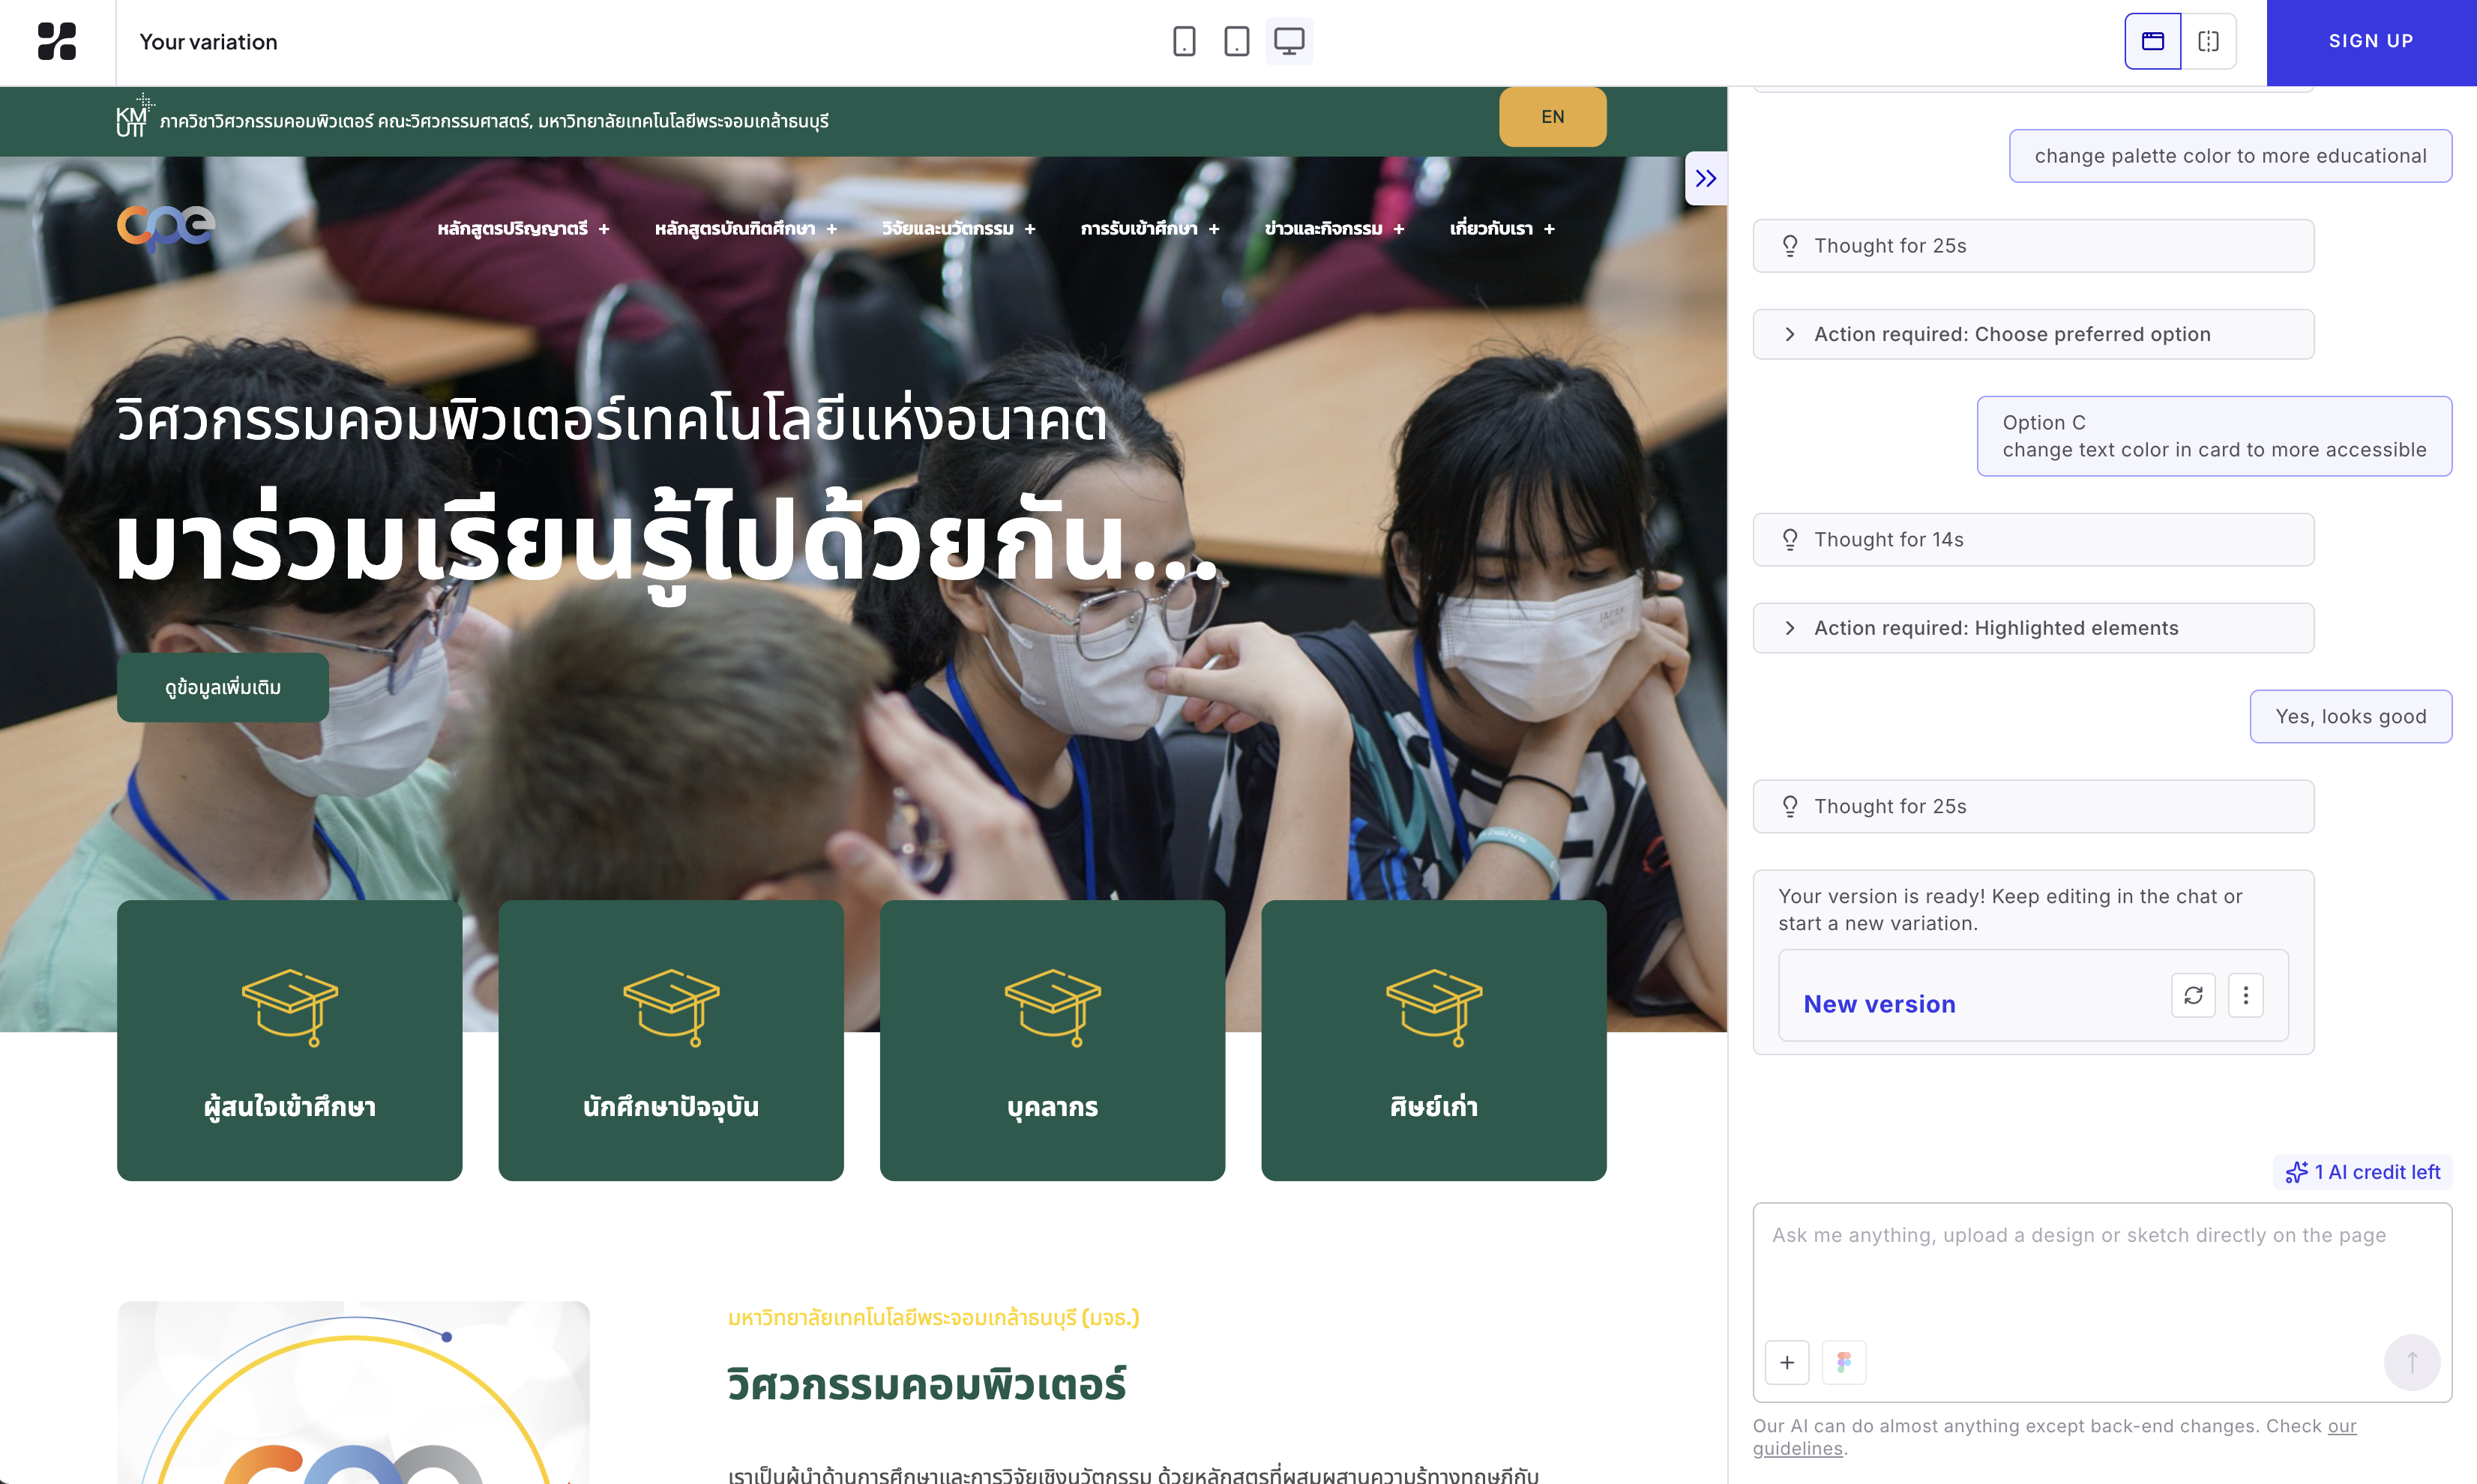
\includegraphics[
          width=0.5\textheight,
          height=0.95\linewidth,
          keepaspectratio,
          origin=c
        ]{figures/ch2-literature-review/kameleoon.png}
        \caption{แพลตฟอร์ม Kameleoon ใช้สำหรับการทำ A/B Testing}
        \label{fig:kameleoon}
      \end{figure}

    \item \textbf{เครื่องมือทดสอบผู้ใช้ก่อนเขียนโค้ด (เช่น Lyssna, Useberry)} มีฟังก์ชัน Preference testing สำหรับเปรียบเทียบดีไซน์หลายแบบ~\cite{lyssna,useberry} และ Lyssna เริ่มมี AI ช่วยสรุปธีมหลักจากคำตอบของผู้เข้าร่วมแล้ว~\cite{lyssna_synthesize} แต่จากการสำรวจเครื่องมือกลุ่มนี้ยังไม่ใช้ AI สร้างทางเลือกการออกแบบ (Variants) และยังไม่แยกปัญหาการใช้งาน (Pain point) ออกจากความชอบของผู้ใช้ในระบบเดียวกัน
      \begin{figure}[H]
        \centering
        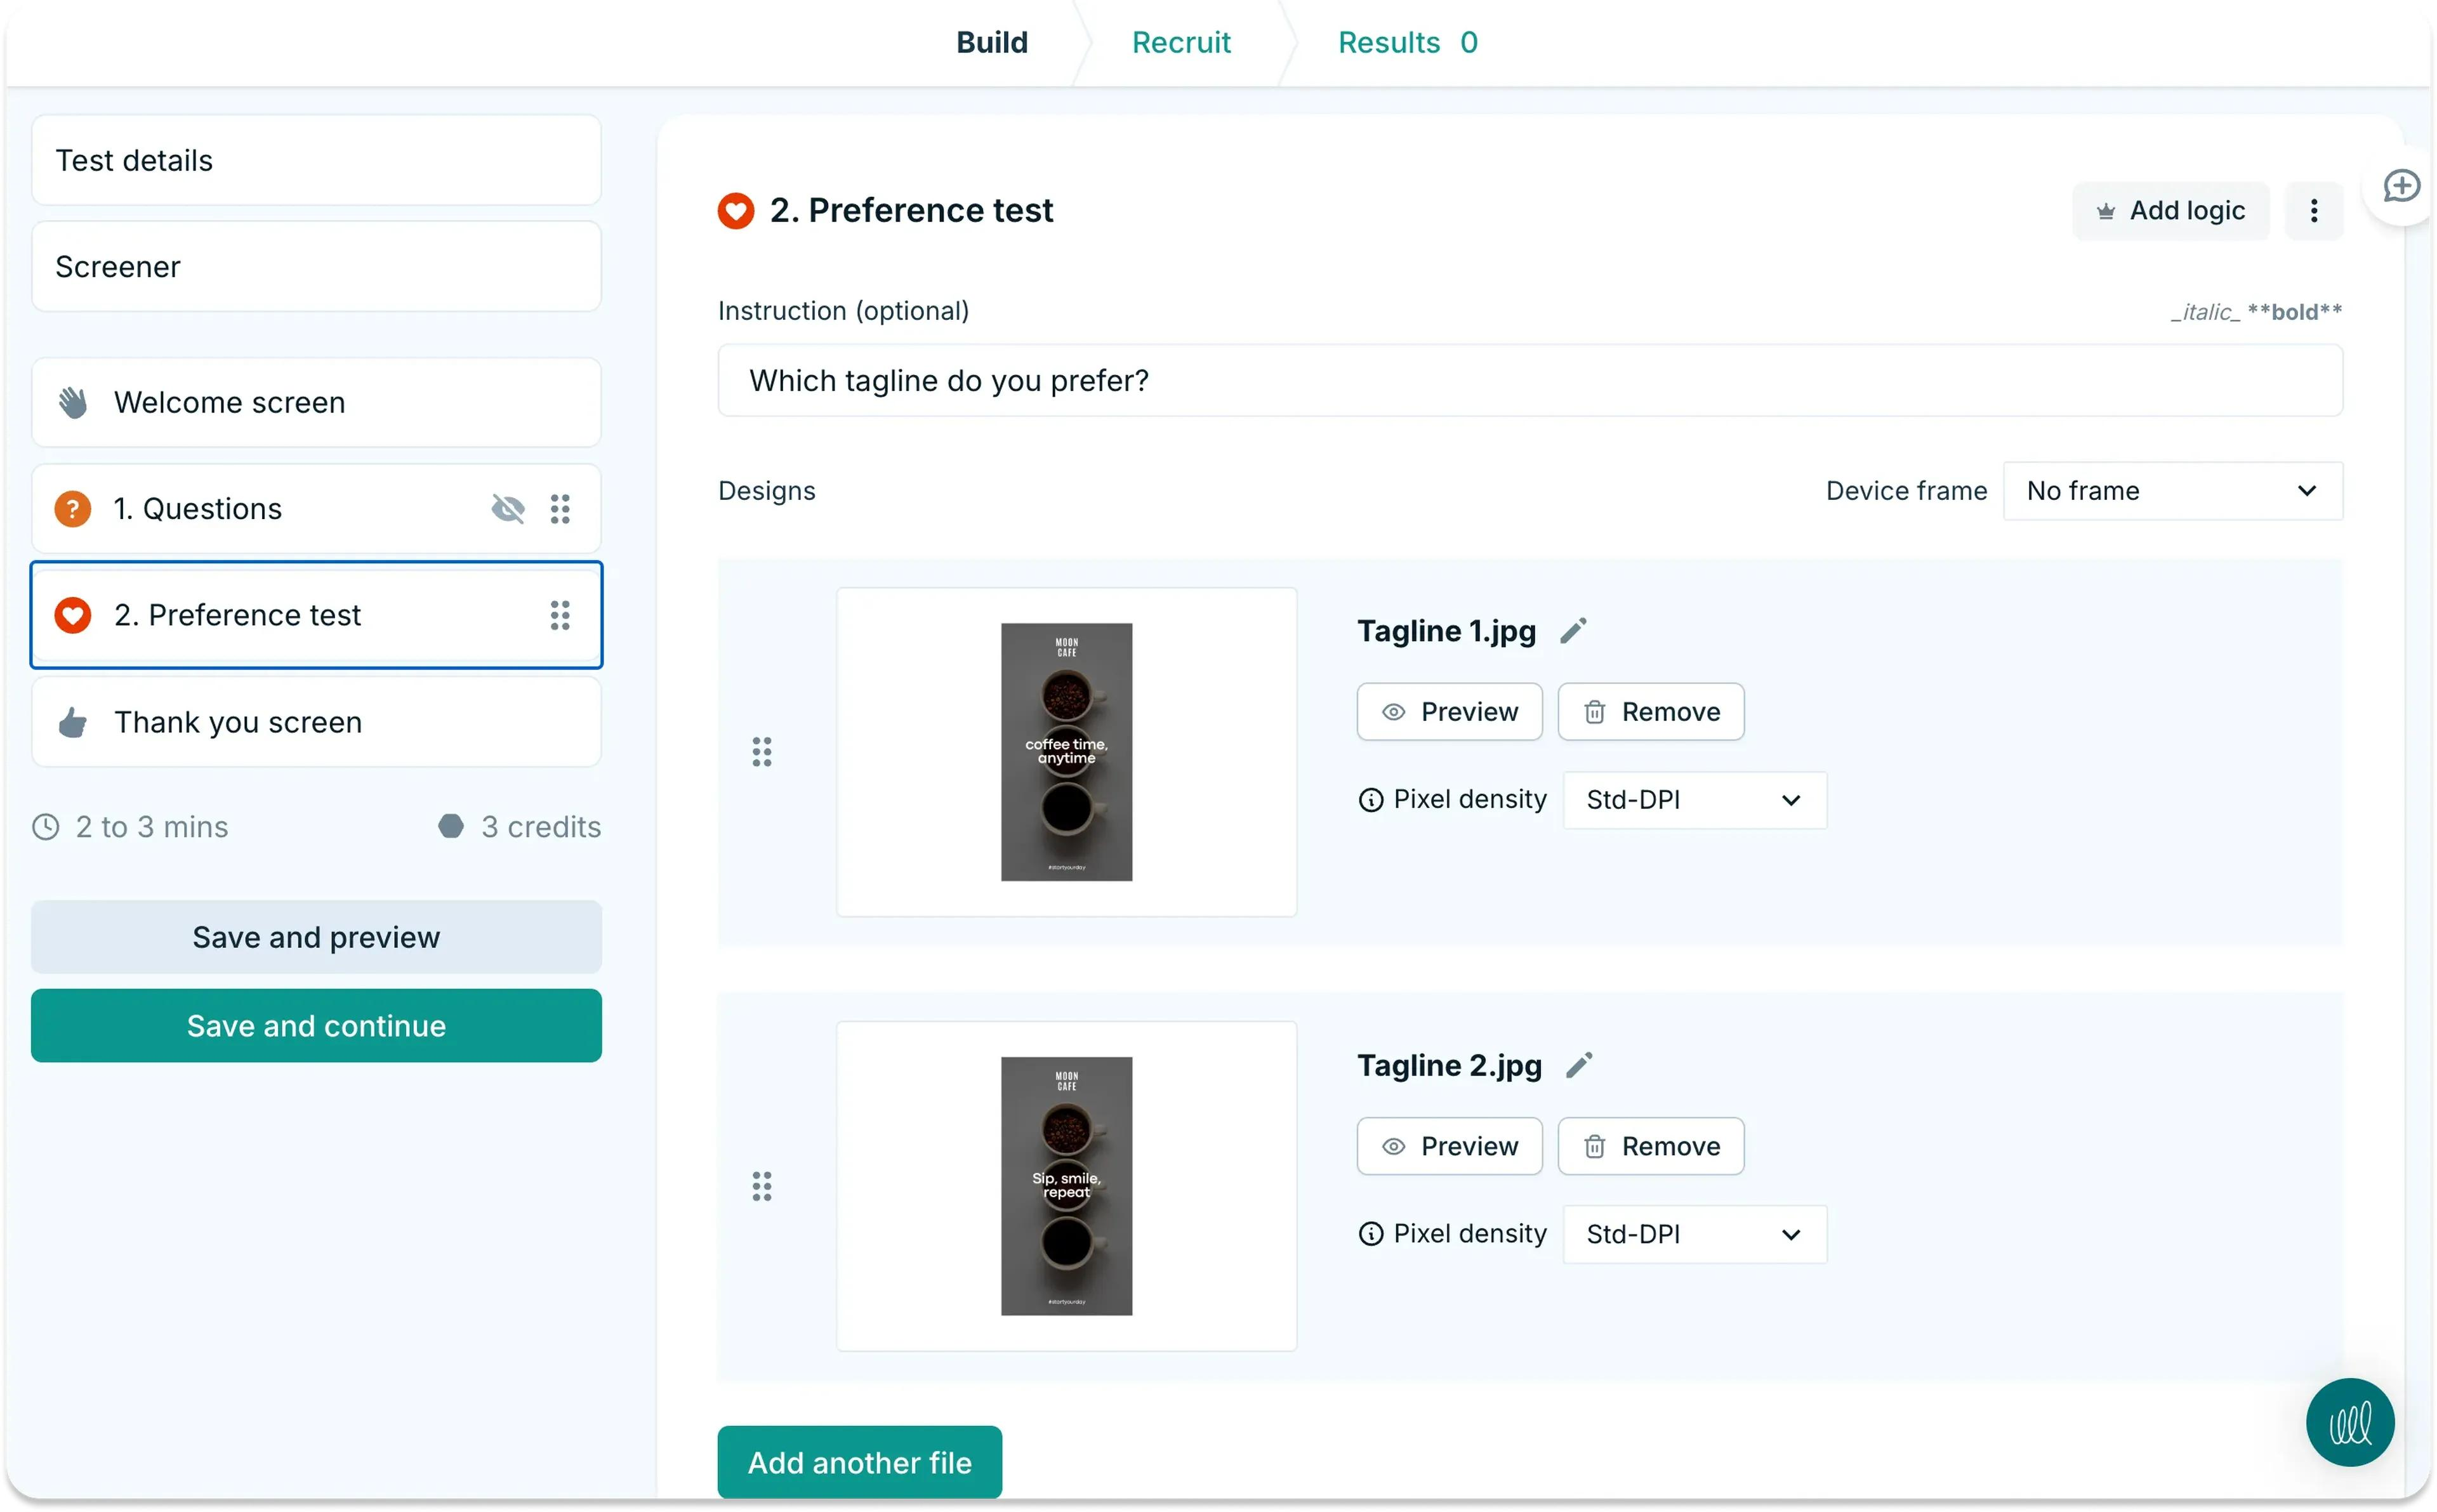
\includegraphics[
          width=0.5\textheight,
          height=0.95\linewidth,
          keepaspectratio,
          origin=c
        ]{figures/ch2-literature-review/lyssna.png}
        \caption{แพลตฟอร์ม Lyssna ใช้สำหรับการทดสอบการใช้งาน}
        \label{fig:lyssna}
      \end{figure}

    \item \textbf{เครื่องมือออกแบบที่มีปัญญาประดิษฐ์เป็นตัวช่วยในการทำงาน (เช่น Figma Make, Figma Agent)} สามารถสร้างต้นแบบหรือ Variants จากคำสั่งได้ โดย agent ของ Figma สร้าง Variants สำหรับ split test จาก component, token และ style ของ Design System~\cite{figma_agent} อย่างไรก็ตาม จากการสำรวจเครื่องมือกลุ่มนี้ยังไม่มีระบบรวบรวมข้อเสนอแนะจากผู้ทดสอบหลายกลุ่มเพื่อนำมาวิเคราะห์ร่วมกัน\cite{figma_agent}
      \begin{figure}[H]
        \centering
        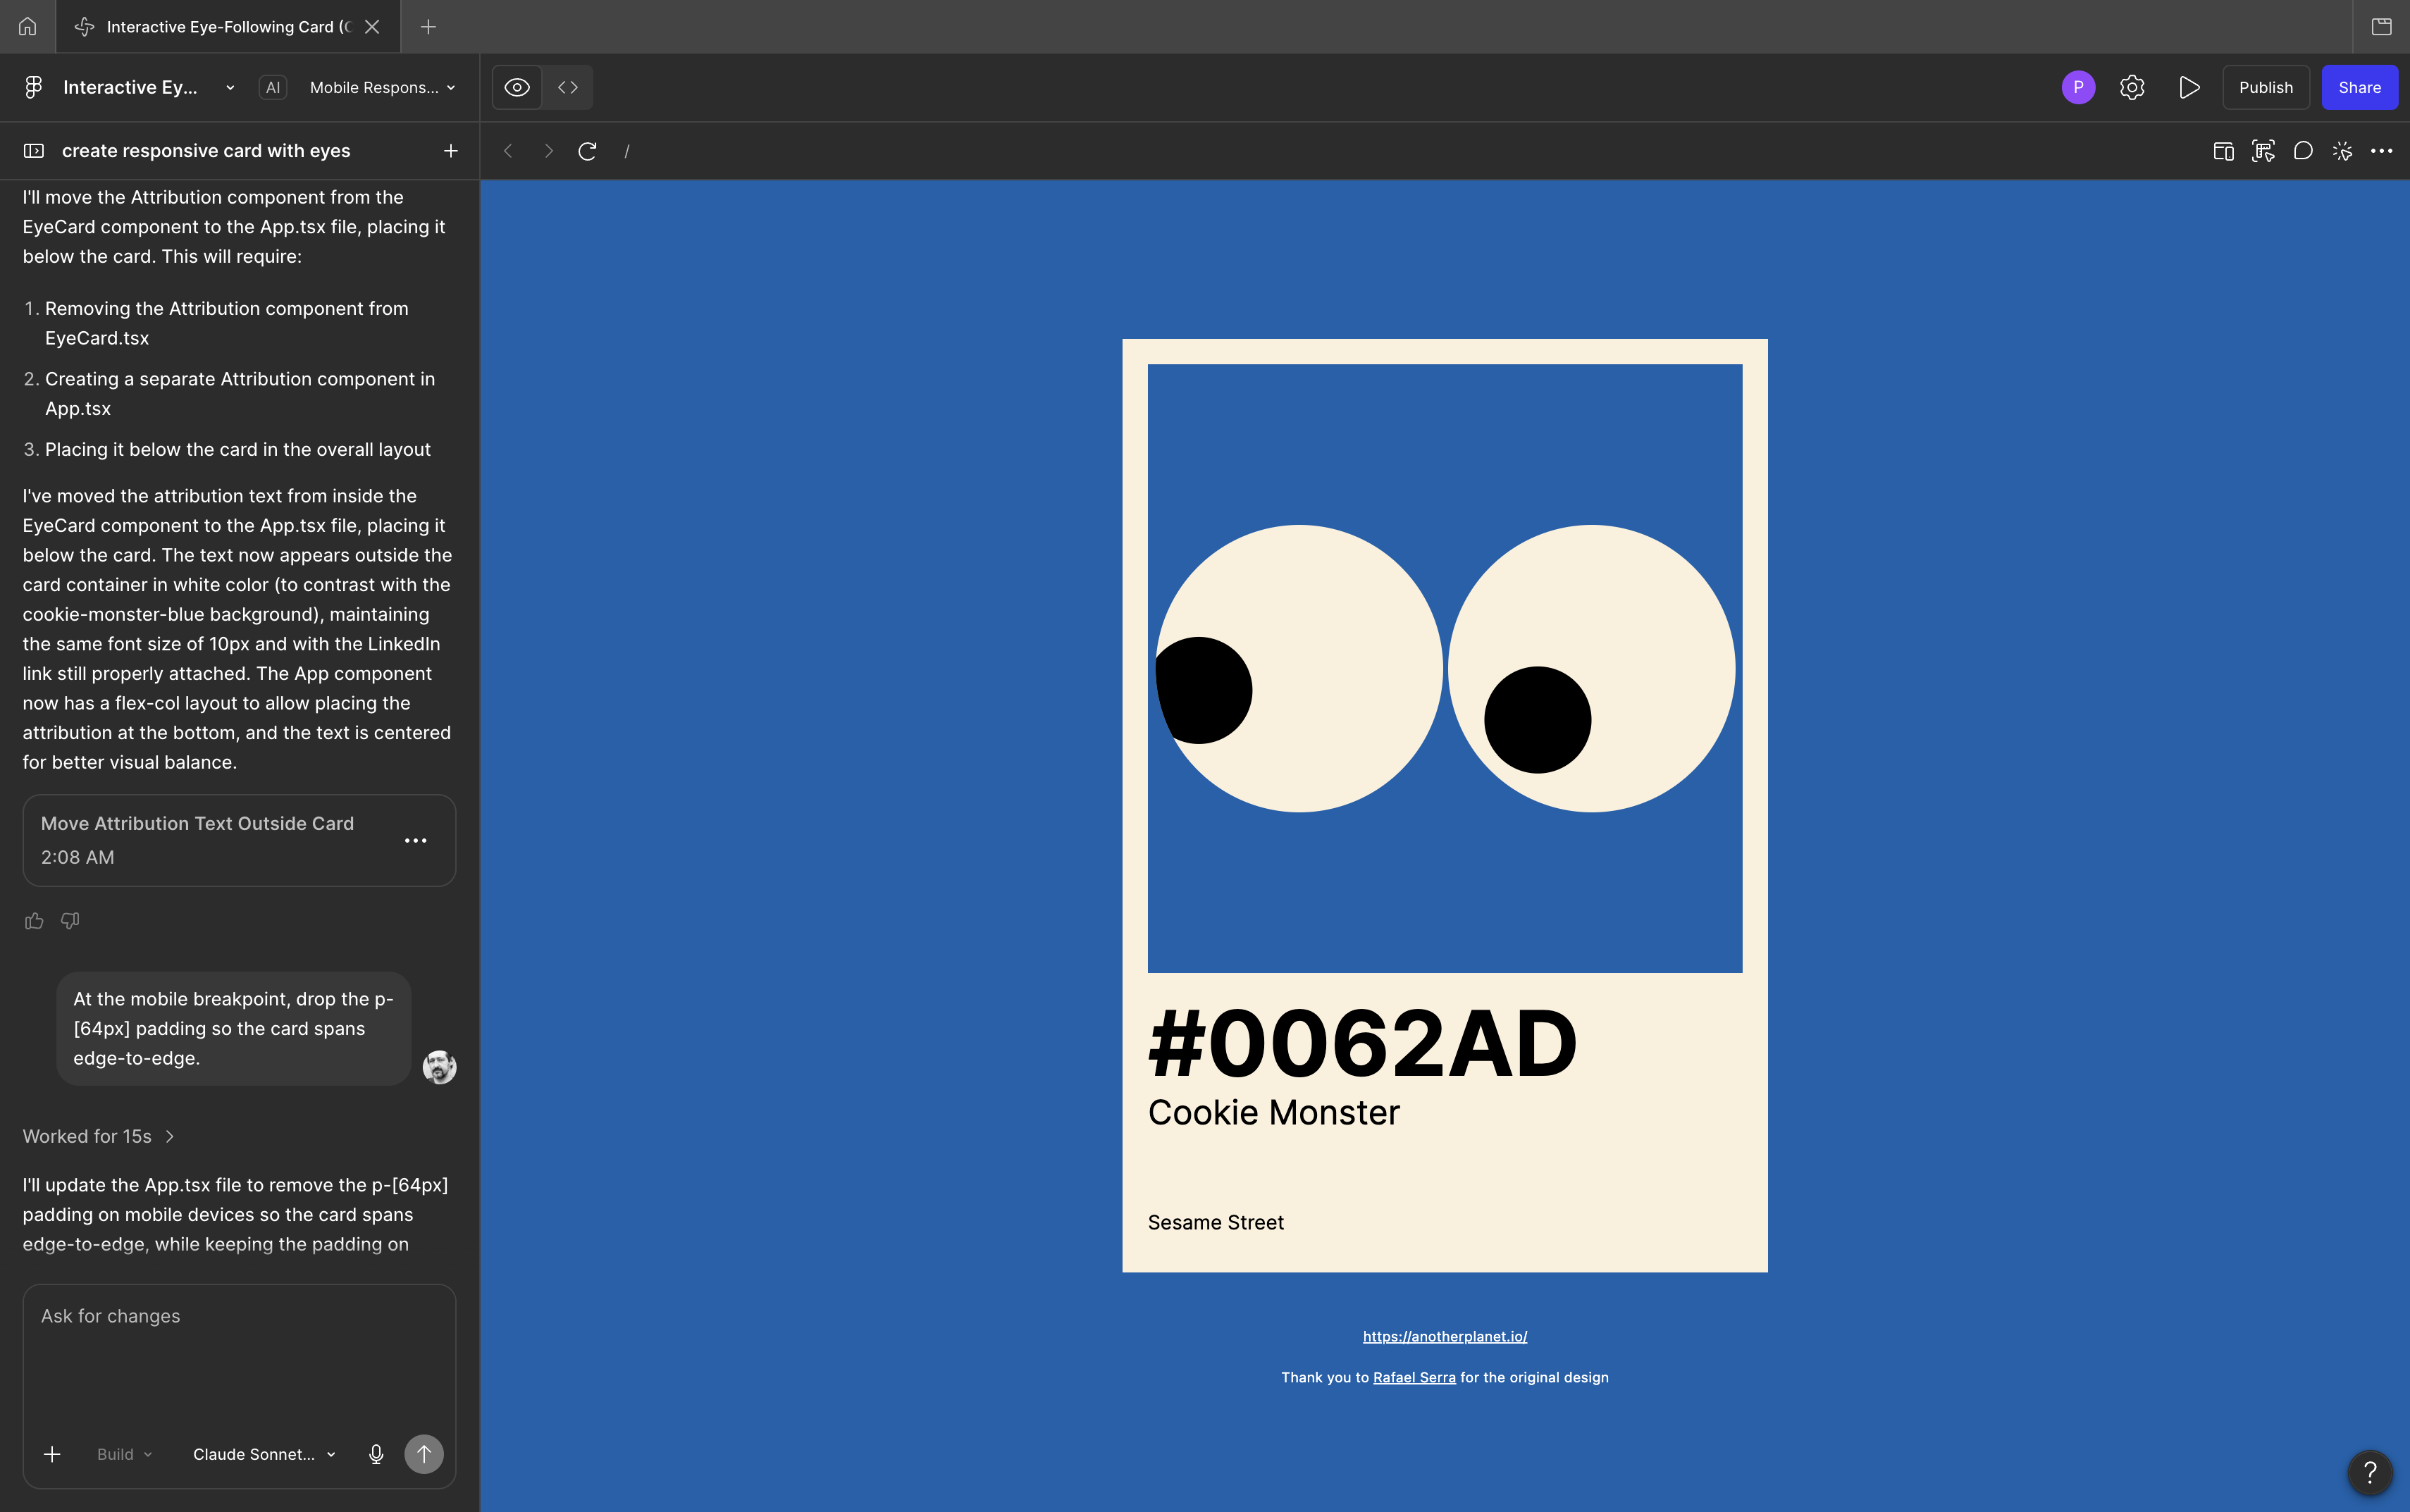
\includegraphics[
          width=0.5\textheight,
          height=0.95\linewidth,
          keepaspectratio,
          origin=c
        ]{figures/ch2-literature-review/figma-make.png}
        \caption{แพลตฟอร์ม Figma Make ใช้สำหรับสร้าง UI ด้วยภาษาธรรมชาติ}
        \label{fig:figma-make}
      \end{figure}

    \item \textbf{เครื่องมือตรวจงานด้วยหมุดคอมเมนต์ (เช่น BugHerd, Marker.io)} ให้ผู้ใช้ปักหมุดความคิดเห็นบนหน้าเว็บ พร้อมแนบภาพหน้าจอและข้อมูลทางเทคนิคโดยอัตโนมัติ~\cite{bugherd,markerio} และเริ่มนำ AI มาใช้จัดการข้อเสนอแนะแล้ว เช่น BugHerd เชื่อมต่อ AI agent ผ่าน MCP เพื่อช่วยคัดแยกงาน~\cite{bugherd_ai} แต่ยังขาดฟังก์ชันเปรียบเทียบสองทางเลือกและการจำแนกข้อเสนอแนะตามประเภทปัญหา
  \end{itemize}
}

\section{ภาษาคอมพิวเตอร์เเละเทคโนโลยี}

\subsection{แบบจำลองภาษาขนาดใหญ่ (Large Language Models: LLM)}

\thaijustify{
  แบบจำลองภาษาขนาดใหญ่ (Large Language Models: LLM) คือ เทคโนโลยีปัญญาประดิษฐ์ที่ฝึกด้วยข้อมูลข้อความจำนวนมาก ทำให้สามารถเข้าใจภาษาธรรมชาติ วิเคราะห์บริบท ให้เหตุผล และสร้างเนื้อหาหรือโค้ดได้ จึงสามารถนำมาช่วยลดภาระงานและสนับสนุนกระบวนการพัฒนาระบบได้อย่างมีประสิทธิภาพ
}

\thaijustify{
  โครงงานนี้ใช้ LLM ผ่าน CPE AI Gateway \cite{cpe_ai_gateway} สำหรับการสร้าง UI และประมวลผลภาษาธรรมชาติ โดยออกแบบกระบวนการแบบ AI Orchestration เพื่อเลือกโมเดลให้เหมาะสมกับแต่ละงาน โมเดลที่นำมาใช้ ได้แก่ muse-glimmer-30b และ qwen3.8-27b พร้อมเปรียบเทียบกับกลุ่ม Frontier Model เพื่อพิจารณาจุดเด่นและความเหมาะสมในการใช้งาน
}

% \thaijustify{
%   muse-glimmer-30b เป็นโมเดล open-weight ขนาดประมาณ 30 พันล้านพารามิเตอร์ที่มีความสมดุลระหว่างความสามารถในการให้เหตุผลและความเร็วในการประมวลผล โดยเฉพาะการสร้างผลลัพธ์แบบมีโครงสร้าง จึงเหมาะกับงาน Prompt-to-Design ที่แปลงคำสั่งภาษาธรรมชาติเป็นโครงสร้าง UI แบบสองทางเลือก (two-alternative UI) อีกทั้งยังใช้ทรัพยากรน้อยกว่าการใช้ Frontier Model ในทุกขั้นตอน \cite{meta2026museglimmer}
% }

\thaijustify{
   muse-glimmer-30b (Muse Glimmer) เป็นโมเดล open-weight ขนาดประมาณ 30 พันล้านพารามิเตอร์จาก Meta Superintelligence Labs ออกแบบมาสำหรับงานเอเจนต์ที่ทำงานต่อเนื่องบนเครื่องภายใน และรันบนฮาร์ดแวร์ระดับผู้บริโภคได้~\cite{meta2026museglimmer}จึงใช้ทรัพยากรน้อยกว่าการเรียกใช้ Frontier Model ในทุกขั้นตอน โครงงานนี้จึงเลือกใช้โมเดลนี้สำหรับงาน Prompt-to-Design ซึ่งแปลงคำสั่งภาษาธรรมชาติเป็นโครงสร้าง UI แบบสองทางเลือก (two-alternative UI)
}

% \thaijustify{
%   qwen3.8-27b เป็นโมเดลขนาด 27 พันล้านพารามิเตอร์ที่เด่นด้านการเข้าใจและประมวลผลภาษาธรรมชาติ จึงเหมาะกับการวิเคราะห์ข้อเสนอแนะจากผู้ทดสอบที่มักเป็นภาษาพูดและไม่มีโครงสร้าง ระบบสามารถใช้โมเดลนี้เพื่อสรุป จัดกลุ่ม และสกัดข้อมูลเชิงลึกจากข้อเสนอแนะเพื่อนำไปสร้าง Persona โดยใช้ทรัพยากรน้อยกว่าโมเดลขนาดใหญ่ \cite{qwentheam2026qwen38}
% }

\thaijustify{
  qwen3.8-27b (Qwen3.8-27B) เป็นโมเดล dense แบบ open-weight ขนาด 27 พันล้านพารามิเตอร์จาก Alibaba เผยแพร่ภายใต้สัญญาอนุญาต Apache~2.0 รับข้อมูลได้ทั้งข้อความ ภาพ และวิดีโอ มี context window 262,144 tokens ซึ่งขยายได้ถึงประมาณ 1 ล้าน tokens~\cite{qwentheam2026qwen38} context ที่ยาวนี้ทำให้ส่งข้อเสนอแนะจำนวนมากจากผู้เข้าร่วมทดสอบหลายคนเข้าไปวิเคราะห์ในคำขอเดียวได้ โครงงานนี้จึงใช้โมเดลนี้สรุป จัดกลุ่ม และสกัดข้อมูลเชิงลึกจากข้อเสนอแนะเพื่อนำไปสร้าง Persona Artifact ทั้งนี้ ผลการประเมินที่เผยแพร่ในช่วงเปิดตัวเป็นตัวเลขที่ผู้พัฒนาโมเดลรายงานเอง จึงต้องประเมินความสามารถของโมเดลกับข้อเสนอแนะภาษาไทย ซึ่งมักเป็นภาษาพูดและไม่มีโครงสร้าง
}

\thaijustify{
  และกลุ่ม Frontier Model มีตัวอย่างในช่วงที่จัดทำโครงงานนี้ ได้แก่ GPT-6 Astra ของ OpenAI ซึ่งเน้นความสามารถด้านการใช้งานคอมพิวเตอร์และวิศวกรรมซอฟต์แวร์ \cite{openai2026gpt6astra} Claude Opus 5.5 ของ Anthropic ซึ่งเน้นงานเขียนโค้ดแบบเอเจนต์ (Agentic Coding) และงานเชิงความรู้ \cite{anthropic2026opus55} และ Gemini 3.8 Flash ของ Google ซึ่งพัฒนาด้านวิศวกรรมซอฟต์แวร์และงานแบบเอเจนต์ โดยยังคงความเร็วสูงและต้นทุนต่ำ \cite{google2026gemini38flash} โมเดลกลุ่มนี้ให้คุณภาพผลลัพธ์สูงในงานที่ซับซ้อน แต่ส่วนใหญ่เป็นโมเดลแบบปิด (Closed-weight) ที่เข้าถึงได้ผ่าน API เชิงพาณิชย์เท่านั้น มีค่าใช้จ่ายตามจำนวนโทเคน และต้องส่งข้อมูลออกไปประมวลผลบนระบบภายนอก ซึ่งเป็นข้อพิจารณาสำคัญเมื่อข้อมูลที่ต้องประมวลผลคือข้อเสนอแนะของผู้เข้าร่วมทดสอบที่อยู่ภายใต้กฎหมายคุ้มครองข้อมูลส่วนบุคคล (PDPA) ด้วยเหตุนี้ โครงงานจึงใช้ Frontier Model เป็นเกณฑ์อ้างอิง (Baseline) ในการประเมินคุณภาพผลลัพธ์ของ muse-glimmer-30b และ qwen3.8-27b แทนการใช้เป็นโมเดลหลักในทุกขั้นตอน
}

\begin{table}[H]
  \centering
  \small
  \caption{เปรียบเทียบความสามารถและจุดด้อยของแบบจำลองภาษาขนาดใหญ่แต่ละรุ่น}
  \label{tab:ai-models-comparison}
  \begin{tabularx}{\textwidth}{
      >{\raggedright\arraybackslash}p{0.20\textwidth}
      |
      >{\raggedright\arraybackslash}X
      >{\raggedright\arraybackslash}X
      >{\raggedright\arraybackslash}X
    }
    \hhline{=|===}
    \textbf{Model} &
    \textbf{ประเภทงาน} &
    \textbf{จุดเด่น} &
    \textbf{จุดด้อย} \\
    \hhline{=|===}
    
    \texttt{muse-glimmer-30b} \newline \textit{(Context: 131K tokens)} &
    Prompt-to-Design และงานที่ต้องใช้การให้เหตุผล &
    มีความสามารถในการทำตามคำสั่งแบบมีโครงสร้าง (Structured output) ได้อย่างแม่นยำ ใช้ทรัพยากรน้อย และตอบสนองรวดเร็ว &
    ความสามารถในการวิเคราะห์ข้อมูลที่ซับซ้อนมาก ๆ หรือความรู้รอบกว้าง ยังเป็นรองโมเดลขนาดใหญ่ (Frontier Models) และมี Context Window ที่จำกัด \\

    \hline
    
    \texttt{qwen3.8-27b} \newline \textit{(Context: 256K - 1M tokens)} &
    การวิเคราะห์ข้อความ การสนทนา และการประมวลผลภาษาธรรมชาติ &
    เข้าใจภาษาพูดและบริบทที่คลุมเครือได้ดีเยี่ยม สรุปใจความ จัดกลุ่มข้อเสนอแนะ และดึงข้อมูลเชิงลึกได้อย่างเป็นธรรมชาติ &
    ขีดความสามารถด้านการคำนวณเชิงตรรกะซับซ้อน หรือการเขียนโค้ดขั้นสูง ยังไม่เทียบเท่ากลุ่ม Frontier Model \\

    \hline

    \texttt{Claude Opus 5.5} \newline \textit{(Frontier Model)} \newline \textit{(Context: 1M tokens)} &
    งานวิเคราะห์เชิงลึกขั้นสูง การเขียนและตรวจสอบโค้ดโปรแกรม &
    มีระบบ Adaptive thinking ที่ช่วยให้เหตุผลได้อย่างละเอียดลึกซึ้ง การใช้งานเครื่องมือ (Tools) มีความเสถียรและแม่นยำสูง &
    มีต้นทุนการเรียกใช้งาน (Cost) ที่ค่อนข้างสูง และระยะเวลาประมวลผล (Latency) อาจใช้เวลานานกว่าโมเดลทั่วไป \\

    \hline
    
    \texttt{Gemini 3.8 Flash} \newline \textit{(Frontier Model)} \newline \textit{(Context: 1M tokens)} &
    งานประมวลผลแบบ Multimodal และงานที่ต้องการผลลัพธ์แบบเรียลไทม์ &
    ประมวลผลได้อย่างรวดเร็วมาก (Fastest output) รองรับการรับข้อมูลทั้งข้อความ ภาพ เสียง และวิดีโอได้ดีเยี่ยมในราคาประหยัด &
    ประสิทธิภาพในการให้เหตุผลเชิงตรรกะสำหรับงานที่ซับซ้อนมาก ๆ อาจยังเป็นรองโมเดลในระดับ Pro หรือระดับที่สูงกว่า \\

    \hline
    
    \texttt{GPT-6 Astra} \newline \textit{(Frontier Model)} \newline \textit{(Context: 1M - 1.1M tokens)} &
    การประสานงานแบบ Multi-agent และการแก้ปัญหาที่ซับซ้อนขั้นสุด &
    มีศักยภาพการให้เหตุผลระดับสูงสุด สามารถควบคุมระบบคอมพิวเตอร์และทำงานซ้อนกันหลายขั้นตอน (Complex reasoning) ได้ดีเยี่ยม &
    มีต้นทุนการใช้งานที่สูงที่สุดในกลุ่ม อาจเกินความจำเป็นสำหรับระบบทั่วไป และมักมีข้อจำกัดด้านโควตาการใช้งานอย่างเข้มงวด \\

    \hline
  \end{tabularx}
\end{table}

% \begin{table}[H]
%   \centering
%   \small
%   \caption{เปรียบเทียบจุดเด่นและจุดด้อยของแบบจำลองภาษาขนาดใหญ่แต่ละรุ่น}
%   \label{tab:ai-models-comparison}
%   \begin{tabularx}{\textwidth}{
%       >{\raggedright\arraybackslash}p{0.20\textwidth}
%       |
%       >{\raggedright\arraybackslash}X
%       >{\raggedright\arraybackslash}X
%       >{\raggedright\arraybackslash}X
%     }
%     \hhline{=|===}
%     \textbf{Model} &
%     \textbf{ประเภทงาน} &
%     \textbf{จุดเด่น} &
%     \textbf{จุดด้อย} \\
%     \hhline{=|===}
 
%     % TODO: ยืนยัน context จาก https://huggingface.co/meta-models/Muse-Glimmer-30B
%     \texttt{muse-glimmer-30b} \newline \textit{(Context: 131K tokens)} &
%     Prompt-to-Design (สร้างและปรับปรุง two-alternative UI) &
%     โมเดล open-weight ขนาด 30B ที่ออกแบบมาสำหรับงานเอเจนต์ รันบนฮาร์ดแวร์ระดับผู้บริโภคได้ จึงใช้ทรัพยากรน้อย~\cite{meta2026museglimmer} &
%     Context window สั้นกว่ากลุ่ม Frontier Model และความแม่นยำในการสร้างผลลัพธ์แบบมีโครงสร้างสำหรับงาน Prompt-to-Design ยังต้องยืนยันด้วยชุดข้อมูลประเมินของโครงงาน \\
 
%     \hline
 
%     \texttt{qwen3.8-27b} \newline \textit{(Context: 262K ขยายได้ถึง 1M tokens)} &
%     การวิเคราะห์ สรุป และจัดกลุ่มข้อเสนอแนะ และการสังเคราะห์ข้อมูลสำหรับ Persona &
%     โมเดล dense แบบ open-weight (Apache~2.0) รับข้อมูลได้ทั้งข้อความ ภาพ และวิดีโอ มี context ยาวพอสำหรับรวมข้อเสนอแนะจำนวนมากในคำขอเดียว~\cite{qwentheam2026qwen38} &
%     ผลประเมินที่เผยแพร่ช่วงเปิดตัวเป็นตัวเลขที่ผู้พัฒนารายงานเอง และความสามารถกับข้อเสนอแนะภาษาไทยแบบภาษาพูดยังต้องประเมินด้วยชุดข้อมูลของโครงงาน \\
 
%     \hline
 
%     % TODO: ยืนยัน context ที่ https://platform.claude.com/docs/en/models/opus-5-5/overview
%     \texttt{Claude Opus 5.5} \newline \textit{(Frontier Model)} \newline \textit{(Context: 1M tokens)} &
%     งานวิเคราะห์เชิงลึก การเขียนโค้ดแบบเอเจนต์ และงานเชิงความรู้ &
%     ผู้พัฒนาระบุว่าเป็นรุ่น Opus ที่ทำงานด้านโค้ด เอเจนต์ และงานเชิงความรู้ได้ดีที่สุด ต้นทุนต่องานต่ำกว่า Opus~5 ราว 40\% และสร้างผลลัพธ์เร็วขึ้นกว่า 30\%~\cite{anthropic2026opus55} &
%     เป็นโมเดลแบบปิด (Closed-weight) ต้องส่งข้อมูลออกไปประมวลผลภายนอก และมีราคา 4/20 ดอลลาร์สหรัฐต่อล้าน tokens (input/output) ซึ่งสูงกว่าโมเดล open-weight มาก \\
 
%     \hline
 
%     % TODO: ยืนยัน context ของรุ่น Flash (หน้า docs ที่พบระบุ 1,048,576 tokens สำหรับรุ่น Flash Cyber)
%     \texttt{Gemini 3.8 Flash} \newline \textit{(Frontier Model)} \newline \textit{(Context: 1M tokens)} &
%     งานวิศวกรรมซอฟต์แวร์ งานแบบเอเจนต์ และงานที่ต้องการผลลัพธ์รวดเร็ว &
%     พัฒนาด้านวิศวกรรมซอฟต์แวร์และงานแบบเอเจนต์ โดยคงความเร็วสูงและต้นทุนต่ำ~\cite{google2026gemini38flash} &
%     % TODO: ช่องนี้ยังไม่มีแหล่งรองรับ
%     ประสิทธิภาพในการให้เหตุผลสำหรับงานที่ซับซ้อนมาก ๆ อาจยังเป็นรองโมเดลระดับ Pro หรือสูงกว่า \\
 
%     \hline
 
%     % TODO: ยืนยัน context จากหน้า model ของ OpenAI API
%     \texttt{GPT-6 Astra} \newline \textit{(Frontier Model)} \newline \textit{(Context: 1M - 1.1M tokens)} &
%     งานที่ใช้คอมพิวเตอร์ (Computer use) วิศวกรรมซอฟต์แวร์ และงานวิชาชีพที่ซับซ้อน &
%     ผู้พัฒนาระบุว่าทำผลงานระดับ state-of-the-art ด้าน computer use, browsing, วิศวกรรมซอฟต์แวร์ และงานวิชาชีพ~\cite{openai2026gpt6astra} &
%     % TODO: ยืนยันราคาจากหน้า pricing ทางการของ OpenAI
%     มีต้นทุนการใช้งานสูงที่สุดในกลุ่ม (10/50 ดอลลาร์สหรัฐต่อล้าน tokens) และอาจเกินความจำเป็นสำหรับระบบทั่วไป \\
 
%     \hline
%   \end{tabularx}
% \end{table}

\thaijustify{
  ในกระบวนการทำงาน AI Orchestration จะเลือกโมเดลตามประเภทของงาน เช่น คำขอที่เกี่ยวข้องกับการสร้างหรือปรับปรุง UI จากความต้องการทางการออกแบบจะถูกส่งไปยัง muse-glimmer-30b ขณะที่งานสนทนา การสรุปและการวิเคราะห์ข้อเสนอแนะ รวมถึงการสังเคราะห์ข้อมูลสำหรับ Persona Artifact จะใช้ qwen3.8-27b เป็นหลัก
}
\thaijustify{
  การแบ่งหน้าที่ดังกล่าวช่วยให้แต่ละโมเดลถูกใช้งานตามความสามารถที่เหมาะสมและทำให้กระบวนการประมวลผลของระบบมีโครงสร้างชัดเจนมากกว่าการใช้โมเดลเดียวสำหรับงานทุกประเภท
}

\subsection{เทคโนโลยีการสร้างส่วนต่อประสานผู้ใช้โดยกำหนด Design System}
\thaijustify{
  งานวิจัยที่ศึกษาการให้ Generative AI สร้าง UI ให้ตรงกับ design system มีการศึกษาเชิงเปรียบเทียบ context engineering สามแบบสำหรับ LLM agent ได้แก่ instruction-based, context-based และ registry-based \cite{designsystem_compliant_ui_2026} ผลพบว่าการให้ agent ใช้ component สำเร็จรูปจาก registry ให้ความสอดคล้องกับ design system สูงและขยายขนาดได้ดีกว่า เพราะเปลี่ยนจากการให้ LLM ตีความข้อความไปเป็นการตรวจสอบระดับ component และมีงานอีกกลุ่มหนึ่งใช้ข้อจำกัดด้านการออกแบบเป็นตัวกำหนด เช่น UIDEC~\cite{uidec_2025} ที่ให้นักออกแบบระบุรายละเอียดโครงการ ได้แก่ วัตถุประสงค์ กลุ่มเป้าหมาย อุตสาหกรรม และสไตล์การออกแบบ แล้วใช้ Generative AI สร้างตัวอย่างการออกแบบที่หลากหลายภายใต้ข้อจำกัดนั้นโดยนักออกแบบแทบไม่ต้องเขียน prompt เอง และ PrototypeFlow~\cite{prototypeflow_humanai_ui_design} ที่สร้าง theme ที่แก้ไขได้และดึงความรู้ด้านการออกแบบมาช่วยให้สี สไตล์ และ layout มีความสอดคล้องกัน จากบทความเหล่านี้ โครงงานนี้จึงนำแนวคิดนี้มาประยุกต์ใช้ในการสร้าง component และ material ที่ทำหน้าที่เป็นโครงสร้างพื้นฐานให้ LLM หรือนักพัฒนาสามารถนำไปหยิบใช้และทำงานต่อได้ทันทีโดยไม่ต้องเสียเวลาเขียนโค้ดหรือจัดการรายละเอียดด้วยตนเองอีกครั้ง
}

\section{สรุปการศึกษาค้นคว้า}

% \begin{table}[H]
%   \centering
%   \small
%   \caption{สรุปประเด็นจากงานวิจัยและเครื่องมือที่เกี่ยวข้อง}
%   \label{tab:literature_summary}
%   \begin{tabularx}{\textwidth}{
%       >{\raggedright\arraybackslash}p{0.18\textwidth}
%       >{\raggedright\arraybackslash}p{0.22\textwidth}
%       >{\raggedright\arraybackslash}X
%       >{\raggedright\arraybackslash}X
%     }
%     \hline
%     \textbf{กลุ่มประเด็น} &
%     \textbf{งานที่เกี่ยวข้อง} &
%     \textbf{สิ่งที่มีการศึกษาแล้ว} &
%     \textbf{ช่องว่างที่พบ} \\
%     \hline

%     การสร้าง UI และต้นแบบด้วย Generative AI &
%     \cite{suh2025storyensemble, feng2023designing, yuan2024towards, kolthoff2024} &
%     Generative AI สามารถช่วยสร้าง wireframe, prototype และทางเลือกของ UI
%     จากความต้องการของนักออกแบบ เพื่อลดเวลาและแรงงานในการสร้างต้นแบบ
%     และช่วยให้สามารถสำรวจทางเลือกของการออกแบบได้มากขึ้น &
%     ผลลัพธ์ที่สร้างโดย Generative AI ยังพบปัญหาด้าน layout, style และการตีความ
%     function ที่ไม่ตรงกับความต้องการ รวมถึงยังไม่ได้เชื่อมกับกระบวนการ
%     ทดสอบและปรับปรุงจากข้อเสนอแนะของผู้ใช้อย่างครบวงจร \\

%     \hline

%     การทดสอบและการสกัดความต้องการจากต้นแบบ &
%     \cite{nielsen2000five, virzi1992refining,
%     nielsen1993mathematical, pacheco2018, lu2026} &
%     การทดสอบกับผู้ใช้กลุ่มเล็กหลายรอบสามารถช่วยค้นพบปัญหาได้อย่างมีประสิทธิภาพ
%     และการใช้ prototype ช่วยให้นักออกแบบสามารถสกัดความต้องการและรับ
%     ข้อเสนอแนะก่อนพัฒนาระบบจริงได้ &
%     การทำการทดสอบซ้ำหลายรอบยังสร้างภาระในการเตรียมหลายรูปแบบของ UI
%     รวบรวมข้อเสนอแนะ และนำผลจากแต่ละรอบกลับไปปรับปรุงการออกแบบ \\

%     \hline

%     การตีความข้อเสนอแนะและการสร้าง User Persona &
%     \cite{nngroup_satisfaction, nngroup_qualitative,
%     shukla2025, mitchell1997, shin2024} &
%     งานวิจัยแสดงให้เห็นว่าความชอบของผู้ใช้อาจไม่ตรงกับปัญหาการใช้งานจริง
%     และข้อเสนอแนะยังแตกต่างกันตามบทบาทและความต้องการของผู้ให้ข้อมูล
%     นอกจากนี้ LLM สามารถช่วยสรุปข้อมูลเพื่อสร้าง User Persona ได้
%     แต่ยังต้องอาศัยมนุษย์ในการระบุและตรวจสอบลักษณะที่สำคัญของผู้ใช้ &
%     ยังต้องมีกระบวนการเชื่อมโยงข้อเสนอแนะกับกลุ่มผู้ใช้
%     แยกความต้องการและความชอบออกจากกัน และนำข้อมูลเหล่านี้ไปสังเคราะห์
%     เป็น Persona ที่นักออกแบบสามารถตรวจสอบและนำกลับไปใช้ในการออกแบบได้ \\

%     \hline

%     การใช้ปัญญาประดิษฐ์วิเคราะห์ข้อเสนอแนะร่วมกับมนุษย์ &
%     \cite{gao2024collabcoder, gebreegziabher2023patat,
%     song2025, amershi2019, pourasad2025} &
%     LLM สามารถช่วยจัดกลุ่ม สรุป และวิเคราะห์ข้อมูลเชิงคุณภาพได้
%     แต่ยังมีข้อจำกัดด้านอคติและอาจพลาดข้อมูลสำคัญ
%     งานวิจัยจึงสนับสนุนการให้มนุษย์เข้ามาตรวจสอบและตัดสินใจร่วมกับปัญญาประดิษฐ์ &
%     จำเป็นต้องมีกระบวนการที่ให้นักออกแบบตรวจสอบ แก้ไข
%     และยืนยันผลการวิเคราะห์ของปัญญาประดิษฐ์ก่อนที่ผลลัพธ์จะถูกนำไปใช้
%     ปรับปรุงงานออกแบบ \\

%     \hline

%     เครื่องมือที่มีอยู่ในปัจจุบัน &
%     \cite{kameleoon, otterab, lyssna, useberry,
%     figma_agent, bugherd, markerio} &
%     เครื่องมือแต่ละประเภทสนับสนุนบางส่วนของกระบวนการ เช่น
%     การทดสอบหลายรูปแบบ การทดสอบ prototype การสร้าง UI ด้วย AI
%     หรือการให้ข้อเสนอแนะบนงานออกแบบ &
%     ความสามารถเหล่านี้ยังแยกอยู่ในหลายเครื่องมือ
%     และยังไม่มีการเชื่อมตั้งแต่การสร้างทางเลือกของ UI
%     การทดสอบ การวิเคราะห์ข้อเสนอแนะ การสร้าง Persona
%     จนถึงการนำผลกลับไปใช้ในรอบการออกแบบถัดไป \\

%     \hline
%   \end{tabularx}
% \end{table}

\thaijustify{
  จากการศึกษางานวิจัยและเครื่องมือที่เกี่ยวข้อง พบว่าแต่ละแนวทางสามารถสนับสนุนบางส่วนของ UX/UI DLC ได้แล้ว แต่กระบวนการตั้งแต่
  การสร้างต้นแบบ การทดสอบกับผู้ใช้ การรวบรวมและวิเคราะห์ข้อเสนอแนะจนถึงการนำข้อมูลกลับไปปรับปรุงการออกแบบยังคงแยกออกจากกัน
}
\thaijustify{
  ดังนั้น โครงงานนี้จึงมุ่งเชื่อมกระบวนการเหล่านี้เข้าด้วยกันโดยใช้ Generative AI ช่วยสร้าง two-alternative UI จากความต้องการทางการออกแบบ แล้วนำไปทำ Comparative Usability Test และให้ผู้เข้าร่วมทดสอบสามารถให้ข้อเสนอแนะลงบน component ได้โดยตรง จากนั้นระบบจะช่วยรวบรวมและวิเคราะห์ข้อเสนอแนะเพื่อค้นหาปัญหา ความต้องการ ความชอบและลักษณะร่วมของผู้ใช้แต่ละกลุ่ม เพื่อนำไปสนับสนุนการสร้าง Persona Artifact โดยให้นักออกแบบเป็นผู้ตรวจสอบและตัดสินใจผลลัพธ์ก่อนนำข้อมูลที่ผ่านการยืนยันแล้วกลับไปใช้ในการสร้างและทดสอบรอบถัดไป
}
\thaijustify{
  แนวทางดังกล่าวทำให้ โครงงานไม่ได้มุ่งใช้ Generative AI เพื่อสร้าง two-alternative UI เพียงอย่างเดียว แต่ใช้ปัญญาประดิษฐ์เพื่อสนับสนุน UX/UI DLC ตั้งแต่การสร้างต้นแบบ การทดสอบการใช้งาน ไปจนถึงการนำความต้องการ
  ของผู้ใช้กลับมาใช้ในการตัดสินใจเชิงออกแบบ โดยยังคงให้นักออกแบบเป็นผู้ควบคุมการตัดสินใจในแต่ละรอบ
}

% \thaijustify{
%   และจากการทบทวนวรรณกรรมทำให้เห็นช่องว่างทางการวิจัย คือ ปัจจุบันยังไม่มีเครื่องมือหรืองานวิจัยใดที่รวบรวมความสามารถทั้ง 4 ด้านไว้ในระบบเดียว ได้แก่ (1) การใช้ปัญญาประดิษฐ์สร้าง two-alternative UI ภายใต้ Design system ที่กำหนด (2) การให้ผู้ทดสอบให้ข้อเสนอแนะ (3) การใช้ปัญญาประดิษฐ์แยกแยะ pain point ออกจากความชอบร่วมกับการตัดสินใจของนักออกแบบ และ (4) การสร้าง Persona Artifact จากผลลัพธ์
% }
% \thaijustify{สิ่งที่โครงงานนี้ควรให้ความสำคัญเป็น คือ การพัฒนาแพลตฟอร์มนี้ให้ครอบคลุมกระบวนการตั้งแต่รับโจทย์ สร้างต้นแบบ รวบรวมข้อเสนอแนะ และวิเคราะห์ผลลัพธ์ เพื่อให้นักออกแบบสามารถส่งมอบงานที่มีการตรวจสอบความต้องการของผู้ใช้ที่แท้จริง พร้อมด้วย design system และต้นแบบที่ลูกค้าพึงพอใจให้นักพัฒนาต่อไปได้อย่างมีประสิทธิภาพ
% }

